\documentclass[12pt,a4paper,oneside]{article}
\usepackage{graphicx}
\usepackage{titlepic}
\usepackage[utf8]{inputenc}
\usepackage[left=1.0in,right=1.0in, top=1in, bottom= 1in]{geometry}
\usepackage{amsfonts}
\usepackage{amssymb}
\usepackage{amsmath}
\usepackage{algorithmicx}
\usepackage{algorithm}
\usepackage{algpseudocode}
\usepackage{fancyhdr}
\usepackage{hyperref}
\usepackage{etoolbox}
\usepackage[nottoc]{tocbibind}
\usepackage{appendix}
\usepackage{multicol}
\usepackage{leftidx}
\graphicspath{{figures/}}
\usepackage{ragged2e}
\usepackage{mathtools}
\usepackage{units}
\usepackage{float}
\usepackage{subcaption}
\usepackage{commath}
\usepackage{pdfpages}
\usepackage{wrapfig}
\usepackage[sorting=none]{biblatex} %biblatex package, bibliography
\usepackage{xcolor}
\usepackage{listings}
\usepackage{dirtytalk}
\usepackage{amsthm}

\newcommand\blankpage{%
    \null
    \thispagestyle{empty}%
    %\addtocounter{page}{-1}%
    \newpage}
 
\theoremstyle{definition}
\newtheorem{definition}{Definition}[section]

\newtheorem{theorem}{Theorem}

\usepackage[none]{hyphenat} % Avoids to go out of margin

\usepackage{subfiles}

\definecolor{codegreen}{rgb}{0,0.6,0}
\definecolor{codegray}{rgb}{0.5,0.5,0.5}
\definecolor{codepurple}{rgb}{0.58,0,0.82}
\definecolor{backcolour}{rgb}{0.95,0.95,0.92}

\lstdefinestyle{mystyle}{
    backgroundcolor=\color{backcolour},   
    commentstyle=\color{codegreen},
    keywordstyle=\color{magenta},
    numberstyle=\tiny\color{codegray},
    stringstyle=\color{codepurple},
    basicstyle=\ttfamily\footnotesize,
    breakatwhitespace=false,         
    breaklines=true,                 
    captionpos=b,                    
    keepspaces=true,                 
    numbers=left,                    
    numbersep=5pt,                  
    showspaces=false,                
    showstringspaces=false,
    showtabs=false,                  
    tabsize=2    
}

\lstset{style=mystyle}


% --------------------------------------------- %
\addbibresource{bibliografia.bib} %Import the bibliography file

\title{Sviluppo di plugin per l'import e preview di fixture virtuali basate su GDTF in Unreal Engine}	        % Title
\author{Luca Sorace}				% Authors separated by \\
\date{\today}									    % Date

% Font size of figure smaller than normal size:
\usepackage{caption}
\captionsetup[figure]{font=small}
%\captionsetup[table]{font=small}

%\usepackage{setspace} % double spacing
\linespread{1.2}

\makeatletter
\let\thetitle\@title
\let\theauthor\@author
\let\thedate\@date
\makeatother

\begin{document}
\sloppy


\begin{titlepage}
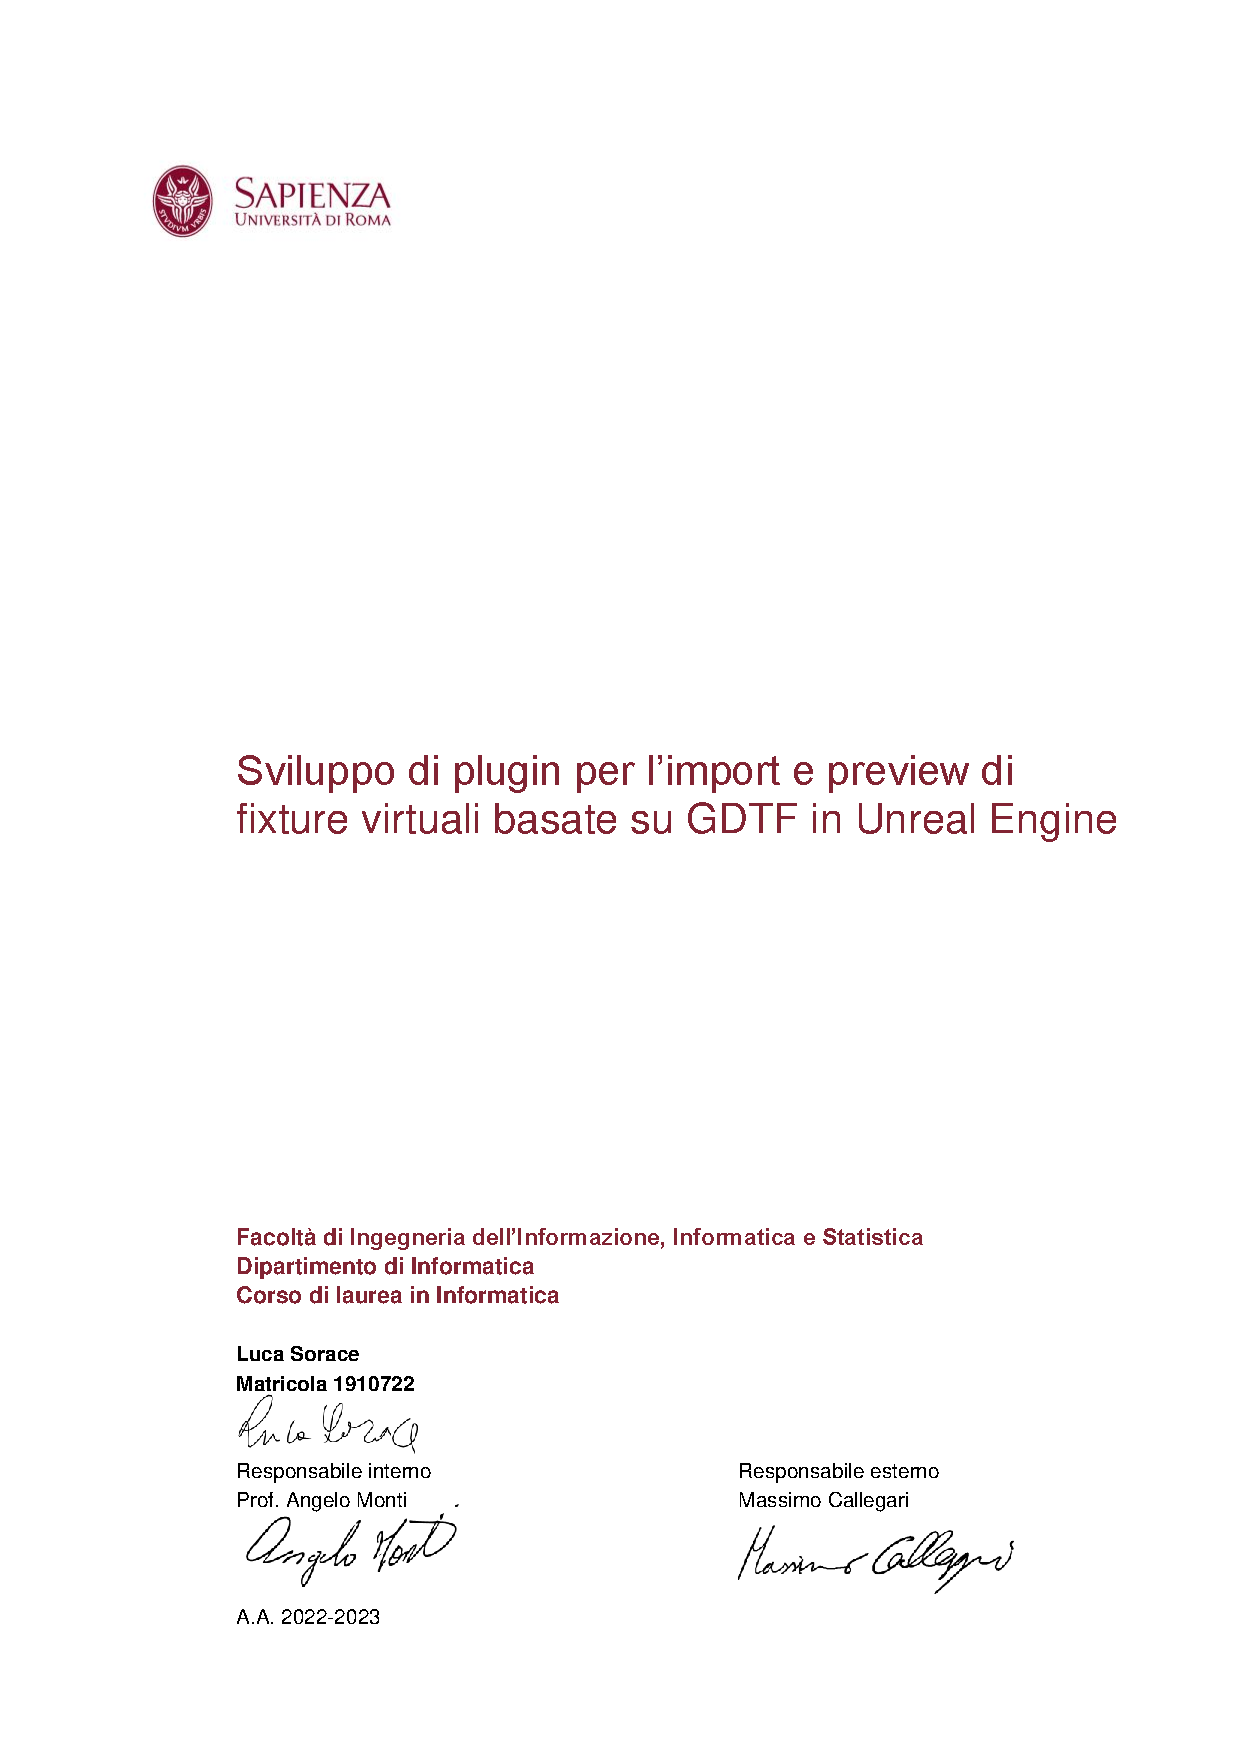
\includepdf[pages=-]{frontespizio.pdf}
\end{titlepage}

\vspace{1.0cm}

% INTRO
% - Anatomia di una fixture
% -- Luci statiche e dinamiche
% -- Moduli di una luce
% -- Protocollo DMX
% - gdtf
% - Informazioni sul tirocinio
% - Strutture dati su Unreal Engine
% - Struttura della tesi
% DESIGN PIPELINE DI RENDERING
% - Vecchia implementazione
% - Idea
% -- Problemi nei custom/material function
% - Generazione del codice (+ ricerca di tutorial su come fare)
% -- Per Beam
% -- Per MF
% REDESIGN GERARCHIA COMPONENTI
% - Vecchia implementazione
% - Idea
% -- Spiegazione strutture dati
% - Implementazione
% -- Ottenimento valori default
% RI-IMPLEMENTAZIONE INTERPOLAZIONE
% - Problemi riscontrati (rapidamente)
% - Implementazione di partenza (Traffic)
% - Modifiche all'implementazione
% -- ((Docs già fatte, vanno tradotte))
% IMPLEMENTAZIONE NUOVE FUNZIONALITA'
% - Sagomatori
% - Iris
% CONCLUSIONI
% - Problemi riscontrati
% - Sviluppi futuri
% -- Arri

\tableofcontents
\clearpage
\newpage
\blankpage
\newpage
\subfile{chapters/01-Introduzione}
\clearpage
\subfile{chapters/02-RenderingPipeline}
\clearpage
\subfile{chapters/03-GerarchiaFixtureComponent}
\clearpage
\subfile{chapters/04-Interpolation}
\clearpage
\subfile{chapters/05-NuoveFeatures}
\clearpage
\subfile{chapters/06-Conclusioni}
\clearpage
\newpage
\blankpage
\printbibliography
\end{document}